\documentclass[tikz]{standalone}
\usepackage{tikz}
\begin{document}

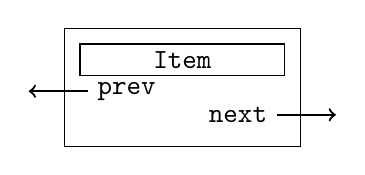
\begin{tikzpicture}[every node/.style={font=\ttfamily}, x=1cm, y=1cm]

% Node 1 (full box)
\draw (0, 0) rectangle (3, 1.5);
\draw (0.2, 0.9) rectangle (2.8, 1.3); % Item box
\node at (1.5, 1.1) {Item};
\node[anchor=west] (prev1) at (0.3, 0.7) {prev}; % prev label
\node[anchor=east] (next1) at (2.7, 0.4) {next};


% NULL

% next arrows (straight)
\draw[->, thick] (next1.east) -- ++(0.75, 0);
\draw[->, thick] (prev1.west) -- ++(-0.75, 0); % to NULL

\end{tikzpicture}

\end{document}
